
The MoRC is the part of the EVC (European vital computer) responsible for the
management of radio communication.
According to the specification this module interacts directly with the following
on-board modules, as shown in figure \ref{fig:arch}: 
\begin{itemize}
\item (DMI) driver module interface~: receives/displays information from/to the driver,
\item (RTM) radio transmission module~: receives/gives commands from/to the radio
network,
\item (BTM) balise transmission module~: sends transmission request from a balise group,
\item (JRU) Juridical recorder unit~: records part of the data exchange for
\item (OBU tasks) other on-board functions (SUBSET-026-4.5) used  by the MoRC such as:
\begin{itemize}
\item track conditions management functions  (SUBSET-026-3.12.1)
that determine for instance if the ETCS system of the track is compatible with the
system on-board.
\item Mode determination (SUBSET-026-3.12.4, SUBSET-026-4.6).

\end{itemize}
\end{itemize}

\begin{figure}[htpb]
\centering
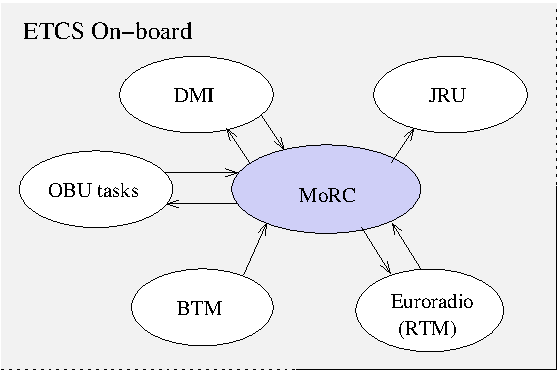
\includegraphics[width =.5\textwidth]{architecture.pdf}
\caption{\label{fig:arch}Interactions between the MoRC and others On-board modules}
\end{figure}

The orders to initiate or terminates a radio communication may come from the
DMI, the BTM, and the RBC (radio block centre) through the RTM. The others OBU
tasks may also order a radio communication (see section \ref{subsec:abstaction}
for more details).

In figure \ref{fig:overview} the MoRC model - \emph{our test model} - is composed
with a the test environment (TE). The inputs and outputs
interfaces are explained in details in section \ref{subsec:inputoutput}.
The test environment abstracts away all the others functions or blocks  which
the SUT may interact with. In our description the test environment is
empty, this means that all possible behavior of the environment may be considered.

\begin{figure}[htpb]
\centering
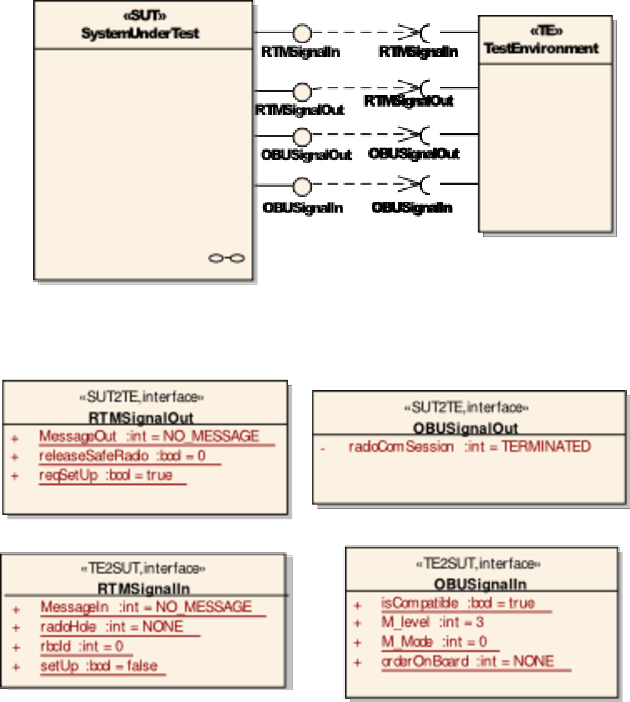
\includegraphics{overview-basicstructure.pdf}
\caption{\label{fig:overview} Model Overview}
\end{figure}

The SUT block consists of two blocks. The SUBSET-026-3.5
specification  separates the management of the radio communication into
3 functions :
\begin{itemize}
\item The session management from chapter 3.5.3 to 3.5.5
\item The registration to the radio network chapter 3.6
\item The safe radio connection indication chapter 3.5.7
\end{itemize}

For the moment we have modeled  the first two items.
The MoRC block and the RadioNetworkRegistration
contains the internal variables used for the protocol implementation and the
state-charts describing their behavior.  The two state machines are
running in parallel.
The two objects interact with each other as shown figure
\ref{fig:sut_interface} and explain later in this document.
\begin{figure}[htpb]
\centering
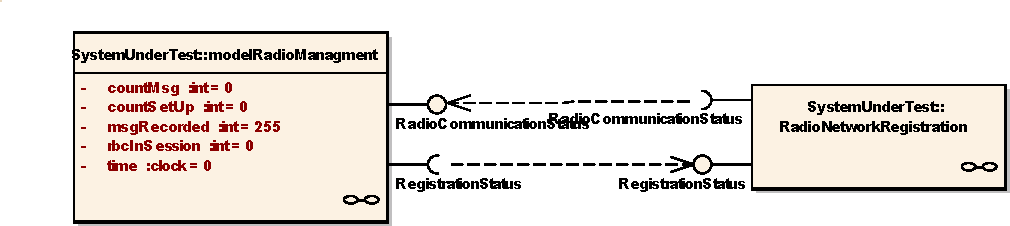
\includegraphics{SystemUnderTest_interface.pdf}
\caption{\label{fig:sut_interface} SUT Overview}
\end{figure}

Until now, the constants used in this chapter and defined in
SUBSET-026.3-A.3.1 are not part of the system under test  block. At this stage of modelisation
it is not defined where they should be declared and recorded to keep track of
possible change or extension. I think they should be part of a special package
regrouping all this kind of information. In the current model they belong to the
system package. 
